% Options for packages loaded elsewhere
\PassOptionsToPackage{unicode}{hyperref}
\PassOptionsToPackage{hyphens}{url}
\PassOptionsToPackage{dvipsnames,svgnames,x11names}{xcolor}
%
\documentclass[
  letterpaper,
  DIV=11,
  numbers=noendperiod]{scrartcl}

\usepackage{amsmath,amssymb}
\usepackage{iftex}
\ifPDFTeX
  \usepackage[T1]{fontenc}
  \usepackage[utf8]{inputenc}
  \usepackage{textcomp} % provide euro and other symbols
\else % if luatex or xetex
  \usepackage{unicode-math}
  \defaultfontfeatures{Scale=MatchLowercase}
  \defaultfontfeatures[\rmfamily]{Ligatures=TeX,Scale=1}
\fi
\usepackage{lmodern}
\ifPDFTeX\else  
    % xetex/luatex font selection
\fi
% Use upquote if available, for straight quotes in verbatim environments
\IfFileExists{upquote.sty}{\usepackage{upquote}}{}
\IfFileExists{microtype.sty}{% use microtype if available
  \usepackage[]{microtype}
  \UseMicrotypeSet[protrusion]{basicmath} % disable protrusion for tt fonts
}{}
\makeatletter
\@ifundefined{KOMAClassName}{% if non-KOMA class
  \IfFileExists{parskip.sty}{%
    \usepackage{parskip}
  }{% else
    \setlength{\parindent}{0pt}
    \setlength{\parskip}{6pt plus 2pt minus 1pt}}
}{% if KOMA class
  \KOMAoptions{parskip=half}}
\makeatother
\usepackage{xcolor}
\setlength{\emergencystretch}{3em} % prevent overfull lines
\setcounter{secnumdepth}{-\maxdimen} % remove section numbering
% Make \paragraph and \subparagraph free-standing
\ifx\paragraph\undefined\else
  \let\oldparagraph\paragraph
  \renewcommand{\paragraph}[1]{\oldparagraph{#1}\mbox{}}
\fi
\ifx\subparagraph\undefined\else
  \let\oldsubparagraph\subparagraph
  \renewcommand{\subparagraph}[1]{\oldsubparagraph{#1}\mbox{}}
\fi


\providecommand{\tightlist}{%
  \setlength{\itemsep}{0pt}\setlength{\parskip}{0pt}}\usepackage{longtable,booktabs,array}
\usepackage{calc} % for calculating minipage widths
% Correct order of tables after \paragraph or \subparagraph
\usepackage{etoolbox}
\makeatletter
\patchcmd\longtable{\par}{\if@noskipsec\mbox{}\fi\par}{}{}
\makeatother
% Allow footnotes in longtable head/foot
\IfFileExists{footnotehyper.sty}{\usepackage{footnotehyper}}{\usepackage{footnote}}
\makesavenoteenv{longtable}
\usepackage{graphicx}
\makeatletter
\def\maxwidth{\ifdim\Gin@nat@width>\linewidth\linewidth\else\Gin@nat@width\fi}
\def\maxheight{\ifdim\Gin@nat@height>\textheight\textheight\else\Gin@nat@height\fi}
\makeatother
% Scale images if necessary, so that they will not overflow the page
% margins by default, and it is still possible to overwrite the defaults
% using explicit options in \includegraphics[width, height, ...]{}
\setkeys{Gin}{width=\maxwidth,height=\maxheight,keepaspectratio}
% Set default figure placement to htbp
\makeatletter
\def\fps@figure{htbp}
\makeatother

\KOMAoption{captions}{tableheading,figureheading}
\makeatletter
\makeatother
\makeatletter
\makeatother
\makeatletter
\@ifpackageloaded{caption}{}{\usepackage{caption}}
\AtBeginDocument{%
\ifdefined\contentsname
  \renewcommand*\contentsname{Tabla de contenidos}
\else
  \newcommand\contentsname{Tabla de contenidos}
\fi
\ifdefined\listfigurename
  \renewcommand*\listfigurename{Listado de Figuras}
\else
  \newcommand\listfigurename{Listado de Figuras}
\fi
\ifdefined\listtablename
  \renewcommand*\listtablename{Listado de Tablas}
\else
  \newcommand\listtablename{Listado de Tablas}
\fi
\ifdefined\figurename
  \renewcommand*\figurename{Figura}
\else
  \newcommand\figurename{Figura}
\fi
\ifdefined\tablename
  \renewcommand*\tablename{Tabla}
\else
  \newcommand\tablename{Tabla}
\fi
}
\@ifpackageloaded{float}{}{\usepackage{float}}
\floatstyle{ruled}
\@ifundefined{c@chapter}{\newfloat{codelisting}{h}{lop}}{\newfloat{codelisting}{h}{lop}[chapter]}
\floatname{codelisting}{Listado}
\newcommand*\listoflistings{\listof{codelisting}{Listado de Listados}}
\makeatother
\makeatletter
\@ifpackageloaded{caption}{}{\usepackage{caption}}
\@ifpackageloaded{subcaption}{}{\usepackage{subcaption}}
\makeatother
\makeatletter
\@ifpackageloaded{tcolorbox}{}{\usepackage[skins,breakable]{tcolorbox}}
\makeatother
\makeatletter
\@ifundefined{shadecolor}{\definecolor{shadecolor}{rgb}{.97, .97, .97}}
\makeatother
\makeatletter
\makeatother
\makeatletter
\makeatother
\ifLuaTeX
\usepackage[bidi=basic]{babel}
\else
\usepackage[bidi=default]{babel}
\fi
\babelprovide[main,import]{spanish}
% get rid of language-specific shorthands (see #6817):
\let\LanguageShortHands\languageshorthands
\def\languageshorthands#1{}
\ifLuaTeX
  \usepackage{selnolig}  % disable illegal ligatures
\fi
\usepackage[]{biblatex}
\addbibresource{../../../../references.bib}
\IfFileExists{bookmark.sty}{\usepackage{bookmark}}{\usepackage{hyperref}}
\IfFileExists{xurl.sty}{\usepackage{xurl}}{} % add URL line breaks if available
\urlstyle{same} % disable monospaced font for URLs
\hypersetup{
  pdftitle={La Empresa como Organización. Promoviendo Valores Cooperativos, Humanos y Sociales},
  pdfauthor={Edison Achalma},
  pdflang={es},
  colorlinks=true,
  linkcolor={blue},
  filecolor={Maroon},
  citecolor={Blue},
  urlcolor={Blue},
  pdfcreator={LaTeX via pandoc}}

\title{La Empresa como Organización. Promoviendo Valores Cooperativos,
Humanos y Sociales}
\usepackage{etoolbox}
\makeatletter
\providecommand{\subtitle}[1]{% add subtitle to \maketitle
  \apptocmd{\@title}{\par {\large #1 \par}}{}{}
}
\makeatother
\subtitle{Explorando la estructura social y el enfoque cooperativo de
las empresas para impactar positivamente en la sociedad}
\author{Edison Achalma}
\date{2023-06-13}

\begin{document}
\maketitle
\ifdefined\Shaded\renewenvironment{Shaded}{\begin{tcolorbox}[boxrule=0pt, borderline west={3pt}{0pt}{shadecolor}, enhanced, interior hidden, sharp corners, breakable, frame hidden]}{\end{tcolorbox}}\fi

\hypertarget{la-empresa-como-organizaciuxf3n-un-enfoque-cooperativo-humano-y-social}{%
\section{La Empresa como Organización: Un Enfoque Cooperativo, Humano y
Social}\label{la-empresa-como-organizaciuxf3n-un-enfoque-cooperativo-humano-y-social}}

La empresa es un tipo específico de organización que se caracteriza por
su estructura social, su enfoque cooperativo y su impacto en la
sociedad. Destacan los valores cooperativos, humanos y sociales que la
empresa promueve en su funcionamiento.

Según varios teóricos, como Etzioni, Hall y Barnard, las organizaciones
son unidades sociales creadas con el propósito de alcanzar metas
específicas. En el caso de la empresa, esta se compone de diversos
factores que interactúan bajo la dirección y supervisión del empresario,
con el objetivo principal de lograr fines económicos a través de la
producción de bienes y servicios.

Las características distintivas de la empresa incluyen:

\begin{enumerate}
\def\labelenumi{\arabic{enumi}.}
\item
  \textbf{Grupo social definido:} La empresa reúne a individuos que
  colaboran en la consecución de sus objetivos comunes.
\item
  \textbf{Sistema cooperativo:} Existe una dinámica de trabajo en equipo
  y colaboración entre los miembros de la organización.
\item
  \textbf{Estructuración, coordinación consciente y orientación a un
  fin:} La empresa se organiza y coordina de manera consciente para
  lograr sus metas establecidas.
\item
  \textbf{Vocación de permanencia:} A diferencia de proyectos
  temporales, la empresa tiene una perspectiva de continuidad y
  estabilidad en el tiempo.
\item
  \textbf{Interacción con el ambiente externo:} La empresa se relaciona
  y se adapta al entorno externo en el que opera, teniendo en cuenta
  factores económicos, legales, sociales y tecnológicos.
\end{enumerate}

\hypertarget{la-empresa-como-sistema-coordinaciuxf3n-y-complejidad}{%
\section{La Empresa como Sistema: Coordinación y
Complejidad}\label{la-empresa-como-sistema-coordinaciuxf3n-y-complejidad}}

Un sistema se define como un conjunto de elementos que están discretos e
interrelacionados entre sí, y que trabajan de manera coordinada para
alcanzar un objetivo común.

La empresa se puede entender como un sistema, que se compone de
elementos interrelacionados y coordinados, con el objetivo común de
lograr resultados específicos. Esta perspectiva sistémica resalta la
importancia de una coordinación consciente en el funcionamiento de la
empresa.

\begin{enumerate}
\def\labelenumi{\arabic{enumi}.}
\item
  \textbf{Conjunto de elementos:} La empresa está compuesta por diversos
  elementos, como personas, recursos, procesos y estructuras
  organizativas, que interactúan entre sí.
\item
  \textbf{Estructura del sistema:} La empresa establece relaciones entre
  oferentes y demandantes, es decir, entre los que ofrecen bienes o
  servicios y los que los demandan.
\item
  \textbf{Plan común:} La empresa define un plan en el que se establecen
  los objetivos que se buscan alcanzar, proporcionando una dirección
  clara a seguir.
\item
  \textbf{Funciones características:} La empresa desempeña funciones de
  transformación, es decir, utiliza los recursos disponibles para
  producir bienes o servicios que satisfacen las necesidades de los
  clientes.
\item
  \textbf{Conjunto de estados o situaciones en el tiempo:} La empresa
  atraviesa diferentes etapas y estados a lo largo de su existencia,
  adaptándose a cambios internos y externos.
\end{enumerate}

Bajo esta perspectiva sistémica, se reconoce que la empresa es un
sistema complejo que requiere una coordinación consciente para alcanzar
sus objetivos. Esto implica establecer una estructura organizativa
eficiente, fomentar una comunicación efectiva, gestionar adecuadamente
los recursos y adaptarse a los cambios del entorno.

Al comprender a la empresa como un sistema, se puede tener una visión
holística de su funcionamiento y tomar decisiones estratégicas más
informadas. Además, se enfatiza la importancia de la coordinación y la
interacción entre los elementos del sistema para lograr resultados
exitosos y sostenibles en el tiempo.

\hypertarget{evoluciuxf3n-histuxf3rica-de-la-empresa-del-feudalismo-al-capitalismo-informacional}{%
\section{Evolución Histórica de la Empresa: Del Feudalismo al
Capitalismo
Informacional}\label{evoluciuxf3n-histuxf3rica-de-la-empresa-del-feudalismo-al-capitalismo-informacional}}

\begin{longtable}[]{@{}
  >{\raggedright\arraybackslash}p{(\columnwidth - 4\tabcolsep) * \real{0.2057}}
  >{\raggedright\arraybackslash}p{(\columnwidth - 4\tabcolsep) * \real{0.2837}}
  >{\raggedright\arraybackslash}p{(\columnwidth - 4\tabcolsep) * \real{0.5106}}@{}}
\toprule\noalign{}
\begin{minipage}[b]{\linewidth}\raggedright
Sistema Económico
\end{minipage} & \begin{minipage}[b]{\linewidth}\raggedright
Tipo de Empresa
\end{minipage} & \begin{minipage}[b]{\linewidth}\raggedright
Estructura Básica
\end{minipage} \\
\midrule\noalign{}
\endhead
\bottomrule\noalign{}
\endlastfoot
Sistema Feudal & Empresa Primitiva & Unidad simple, de base familiar \\
Capitalismo Mercantilista & Empresa Comercial & Unidad simple,
organizada, no siempre de base familiar \\
Capitalismo Industrial & Empresa Industrial & Unidad compleja,
organizada, societaria y funcional \\
Capitalismo Financiero & Empresa de Organización Financiera & Unidad
compleja, organizada, multisocietaria, divisional y multinacional \\
Capitalismo de la Información & Empresa de Organización del Conocimiento
& Unidad compleja evolucionada, organizada, multisocietaria y global \\
\end{longtable}

\begin{enumerate}
\def\labelenumi{\arabic{enumi}.}
\item
  \textbf{Sistema Feudal - Empresa Primitiva}: En el sistema feudal, se
  caracterizaba por la existencia de unidades económicas y productivas
  básicas llamadas empresas primitivas. Estas empresas eran unidades
  simples y de base familiar, donde las actividades económicas se
  centraban en la subsistencia y estaban vinculadas a la tierra y a la
  agricultura.
\item
  \textbf{Capitalismo Mercantilista - Empresa Comercial}: Durante el
  periodo del capitalismo mercantilista, surgieron las empresas
  comerciales. Estas empresas eran unidades técnicas-económicas que se
  dedicaban al comercio, tanto a nivel local como internacional. Eran
  organizaciones simples, pero más estructuradas que las empresas
  primitivas, y su objetivo principal era obtener beneficios a través de
  las actividades comerciales.
\item
  \textbf{Capitalismo Industrial - Empresa Industrial}: Con la llegada
  del capitalismo industrial, se desarrollaron las empresas
  industriales. Estas empresas se caracterizaban por ser unidades
  económicas de producción en las que se llevaban a cabo actividades
  industriales y se utilizaban tecnologías avanzadas. Eran unidades
  complejas, organizadas en forma societaria y funcional, con el
  objetivo de maximizar la producción y obtener beneficios.
\item
  \textbf{Capitalismo Financiero - Empresa de Organización Financiera}:
  En el capitalismo financiero, surgieron las empresas de organización
  financiera. Estas empresas se centraban en la gestión y dirección de
  los recursos financieros, tomando decisiones sobre inversiones,
  financiamiento y dirección estratégica. Eran unidades complejas,
  organizadas en forma multisocietaria, divisional y multinacional, con
  un enfoque en la maximización de los beneficios a través de la gestión
  financiera.
\item
  \textbf{Capitalismo de la Información - Empresa de Organización del
  Conocimiento}: En la era del capitalismo de la información, se
  destacan las empresas de organización del conocimiento. Estas empresas
  se centran en el manejo y utilización de la información como recurso
  estratégico, tomando decisiones basadas en el conocimiento y la
  tecnología. Son unidades complejas evolucionadas, organizadas en forma
  multisocietaria y global, con un enfoque en la creación, gestión y
  utilización del conocimiento para obtener ventajas competitivas.
\end{enumerate}

\hypertarget{elementos-constitutivos-de-la-empresa}{%
\section{Elementos constitutivos de la
empresa}\label{elementos-constitutivos-de-la-empresa}}

La empresa está compuesta por diversos elementos que desempeñan un papel
fundamental en su funcionamiento y desarrollo. A continuación, se
detallan los elementos constitutivos de la empresa:

\begin{figure}[H]

{\centering 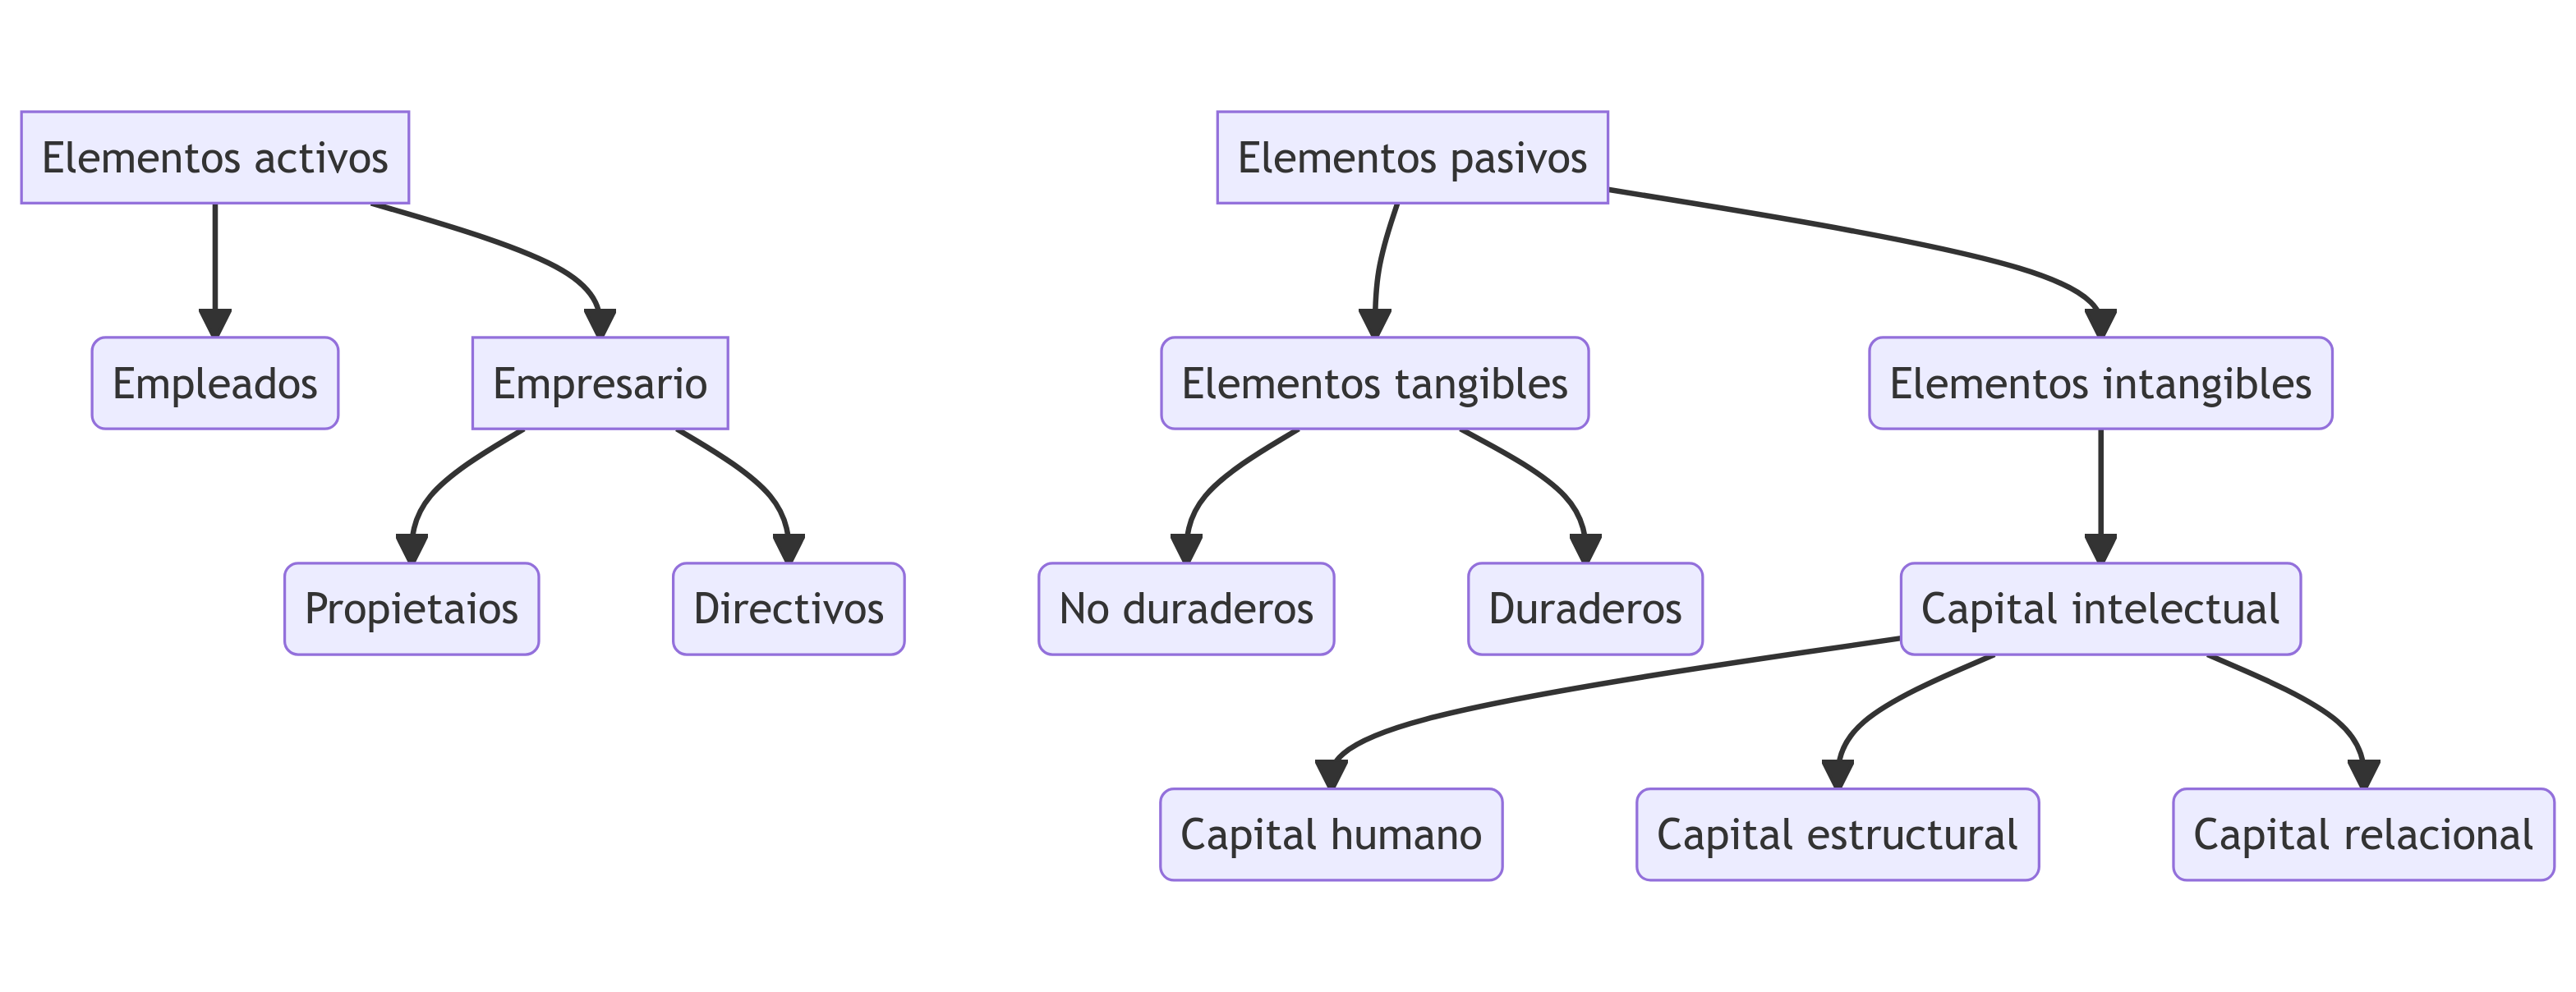
\includegraphics[width=9.98in,height=3.15in]{index_files/figure-latex/mermaid-figure-1.png}

}

\end{figure}

\hypertarget{elementos-activos}{%
\subsection{Elementos activos}\label{elementos-activos}}

\hypertarget{empresario}{%
\subsubsection{Empresario}\label{empresario}}

El empresario es aquel que asume el riesgo y la responsabilidad de la
empresa. Puede ser el propietario o un directivo que toma decisiones
estratégicas y dirige las operaciones de la empresa.

\hypertarget{empleados}{%
\subsubsection{Empleados}\label{empleados}}

Los empleados son el recurso humano que trabaja en la empresa. Estos
desempeñan diferentes roles y funciones dentro de la organización,
contribuyendo al logro de los objetivos empresariales.

\hypertarget{elementos-pasivos}{%
\subsection{Elementos pasivos}\label{elementos-pasivos}}

\hypertarget{elementos-tangibles}{%
\subsubsection{Elementos Tangibles}\label{elementos-tangibles}}

Los elementos tangibles se refieren a los activos físicos de la empresa.
Estos pueden ser no duraderos, como materias primas o productos en
proceso, o duraderos, como maquinaria, equipos y edificios.

\hypertarget{elementos-intangibles}{%
\subsubsection{Elementos Intangibles}\label{elementos-intangibles}}

Los elementos intangibles se refieren a los activos no físicos de la
empresa, que no se pueden tocar ni ver. como el:

Capital Intelectual: Representa el conocimiento y los recursos
intelectuales de la empresa.

\begin{enumerate}
\def\labelenumi{\alph{enumi}.}
\item
  \textbf{Capital Humano:} Se refiere a las competencias y capacidades
  de los empleados, incluyendo su formación, experiencia y habilidades.
\item
  \textbf{Capital Estructural:} Engloba la organización y la tecnología
  utilizada en la empresa, incluyendo los sistemas de gestión, la
  infraestructura tecnológica y los procesos operativos.
\item
  \textbf{Capital Relacional:} Hace referencia a las relaciones que la
  empresa establece con clientes, proveedores y otros agentes del
  entorno empresarial. Estas relaciones son clave para el desarrollo de
  alianzas estratégicas, la colaboración y la creación de redes de
  valor.
\end{enumerate}

\hypertarget{funciuxf3n-de-la-empresa-en-la-economuxeda}{%
\section{Función de la empresa en la
economía}\label{funciuxf3n-de-la-empresa-en-la-economuxeda}}

La empresa desempeña un papel fundamental en la economía al generar
bienes y servicios de forma eficiente. A continuación, se detallan las
funciones principales de la empresa en la economía:

\hypertarget{generar-bienes-y-servicios-de-forma-eficiente}{%
\subsection{Generar bienes y servicios de forma
eficiente}\label{generar-bienes-y-servicios-de-forma-eficiente}}

La empresa tiene como objetivo principal producir bienes y servicios de
manera eficiente, utilizando los recursos disponibles de manera óptima.
Esto implica minimizar los costos de producción y maximizar la calidad y
la productividad.

\hypertarget{asumir-y-reducir-costos-de-mercado-y-de-informaciuxf3n}{%
\subsection{Asumir y reducir costos de mercado y de
información}\label{asumir-y-reducir-costos-de-mercado-y-de-informaciuxf3n}}

La empresa asume y reduce los costos de mercado al organizar la
producción de bienes y servicios de manera interna, en lugar de
adquirirlos a través del mercado. Al hacerlo, la empresa puede
aprovechar economías de escala, especialización y eficiencia en la
producción.

Además, la empresa también asume y reduce los costos de información al
tener acceso a información privilegiada y especializada sobre el
mercado, los consumidores y los proveedores. Esto le permite tomar
decisiones informadas y estratégicas para mejorar su desempeño y
competitividad.

\hypertarget{anticipar-el-producto-obtenido}{%
\subsection{Anticipar el producto
obtenido}\label{anticipar-el-producto-obtenido}}

La empresa tiene la capacidad de anticipar el producto obtenido al
identificar y satisfacer las necesidades y demandas de los consumidores.
A través de la investigación de mercado y el análisis de las tendencias,
la empresa puede desarrollar productos y servicios que se ajusten a las
preferencias del público objetivo, anticipándose así a sus deseos y
expectativas.

\hypertarget{asumir-el-riesgo-de-la-actividad-econuxf3mica}{%
\subsection{Asumir el riesgo de la actividad
económica}\label{asumir-el-riesgo-de-la-actividad-econuxf3mica}}

La empresa asume el riesgo de la actividad económica al invertir
recursos financieros, humanos y tecnológicos en la producción de bienes
y servicios. Esto implica enfrentar la incertidumbre del mercado, los
cambios en la demanda, la competencia y otros factores externos que
pueden afectar su desempeño. La empresa asume este riesgo con el
objetivo de obtener beneficios y lograr su supervivencia en el mercado.

\hypertarget{desarrollar-el-sistema-econuxf3mico}{%
\subsection{Desarrollar el sistema
económico}\label{desarrollar-el-sistema-econuxf3mico}}

La empresa juega un papel crucial en el desarrollo del sistema económico
al generar empleo, contribuir al crecimiento económico, fomentar la
innovación y la investigación, y promover el intercambio comercial. La
actividad empresarial impulsa el desarrollo económico de una sociedad al
generar riqueza, crear oportunidades y estimular la competencia.

\hypertarget{coordinar-el-proceso-productivo}{%
\subsection{Coordinar el proceso
productivo}\label{coordinar-el-proceso-productivo}}

La empresa desempeña un papel de coordinación en el proceso productivo
al organizar y supervisar las diferentes etapas de producción. Esto
implica la planificación, la asignación de recursos, la gestión de
inventarios, la coordinación de equipos de trabajo y el control de la
calidad, entre otras actividades. La empresa busca garantizar la
eficiencia y la coherencia en el proceso productivo para lograr la
satisfacción de los clientes y la obtención de resultados óptimos.

\hypertarget{fundamentos-econuxf3micos-de-las-empresas}{%
\section{Fundamentos económicos de las
empresas}\label{fundamentos-econuxf3micos-de-las-empresas}}

Según Gregory Mankiw, la economía se ocupa del estudio de cómo la
sociedad administra sus recursos. En el contexto de las empresas,
existen diferentes tipos de recursos que son fundamentales para su
funcionamiento. A continuación, se detallan estos recursos y su relación
con la producción de bienes y servicios:

\hypertarget{recursos-naturales}{%
\subsection{Recursos Naturales}\label{recursos-naturales}}

Los recursos naturales son elementos que no son producidos por el ser
humano y que se encuentran disponibles en la naturaleza. Ejemplos de
recursos naturales incluyen terrenos, bosques, agua, minerales,
petróleo, entre otros. Estos recursos son utilizados por las empresas en
sus procesos de producción para extraer, transformar o utilizar como
insumos en la elaboración de bienes y servicios.

\hypertarget{recursos-humanos-o-mano-de-obra}{%
\subsection{Recursos Humanos o Mano de
obra}\label{recursos-humanos-o-mano-de-obra}}

Los recursos humanos se refieren a las capacidades físicas y mentales
que las personas aplican en la producción de bienes y servicios. Esto
incluye tanto el trabajo manual como el trabajo intelectual realizado
por los empleados de una empresa. Los recursos humanos son esenciales
para llevar a cabo las diferentes tareas y funciones necesarias en la
producción y operación de la empresa.

\hypertarget{recursos-financieros-o-capital}{%
\subsection{Recursos Financieros o
Capital}\label{recursos-financieros-o-capital}}

Los recursos financieros, también conocidos como capital, se refieren a
los fondos con los que se adquieren los recursos naturales y humanos
necesarios para la elaboración de productos. El capital puede provenir
de diversas fuentes, como inversionistas, préstamos bancarios, capital
propio de los empresarios, entre otros. Estos recursos financieros se
utilizan para financiar la adquisición de activos, como maquinaria,
equipos, tecnología, así como para cubrir los costos operativos y de
producción de la empresa.

\hypertarget{producciuxf3n-de-bienes-y-servicios}{%
\subsection{Producción de bienes y
servicios}\label{producciuxf3n-de-bienes-y-servicios}}

La producción de bienes y servicios es el resultado de combinar los
recursos naturales, recursos humanos y recursos financieros. En este
proceso, los recursos naturales se utilizan como insumos, los recursos
humanos aportan su trabajo y conocimiento, y los recursos financieros
permiten adquirir y utilizar eficientemente los otros recursos. La
producción de bienes y servicios es el objetivo principal de las
empresas, donde se busca transformar los insumos en productos finales
que satisfagan las necesidades y demandas de los consumidores.

\hypertarget{publicaciones-similares}{%
\section{Publicaciones Similares}\label{publicaciones-similares}}

Aquí te recomendamos algunas publicaciones similares que podrían ser de
tu interés:

\begin{itemize}
\item
  \href{../2023-06-12-introducion-organizacion-industrial/index.qmd}{1.
  Introducción a organización industrial}
\item
  \href{../2023-06-13-empresa-como-organizacion/index.qmd}{2. La Empresa
  como Organización. Promoviendo Valores Cooperativos, Humanos y
  Sociales}
\item
  \href{../2023-06-13-sistemas-economicos/index.qmd}{3. Introducción a
  los Sistemas Económicos. Cómo se distribuyen los recursos y se
  producen}
\item
  \href{../2023-06-15-mercado-relevante-oi-cap-2/index.qmd}{4. El
  Mercado Relevante Industrial de Bienes y el Mercado Geográfico}
\item
  \href{../2023-06-16-concentracion-poder-oi-cap3/index.qmd}{5. Medidas
  de concentracion}
\item
  \href{../2023-06-17-estructura-mercado-oi-cap4/index.qmd}{6.
  Estructura de mercado}
\end{itemize}

Esperamos que encuentres estas publicaciones igualmente interesantes y
útiles. ¡Disfruta de la lectura!


\printbibliography


\end{document}
